\section{Introduction}\label{sec:intro}

A benchmark reports that a new model scores $0.05$ higher than the model it replaces.
What has the new model learned? The question sounds like bookkeeping, but it is a
statistical estimation problem, and the reported number does not answer it whenever the
labels are partly determined by a feature that both models can see.

A concrete case makes the difficulty visible. In relation prediction on Visual Genome
\citep{krishna2017visual}, the task is to name the relation between two objects in an
image, and the pair of object classes already predicts the relation strongly: given
(\textsf{man}, \textsf{surfboard}), the label is very often \textsf{riding}. Two models
that both observe the object classes can therefore differ in their scores for two quite
different reasons. One is that the new model estimates the conditional label frequencies
$\Pr(Y\mid \text{class pair})$ more accurately --- a real improvement, but one that a
lookup table of training frequencies also achieves, and one that evaporates if the
relation frequencies shift. The other is that the new model does better at telling
\emph{these two men on surfboards apart}: it puts higher probability on the correct
label for the individual case, beyond what the class pair alone implies. The reported
score difference is the sum of the two, and no amount of significance testing on that
difference will split it, because the two components are both present in the same
number. The same structure recurs wherever a benchmark has strong label priors: in
visual question answering the form of the question predicts the answer
\citep{agrawal2018dont}, and in long-tailed recognition the class frequencies dominate
aggregate accuracy \citep{ma2024geometric}.

The customary remedy is to build a prior-only reference --- fit
$\widehat\Pr(Y\mid \phi)$ from training data, score it, and see how far the full models
beat it \citep{zellers2018neural}. That is a useful diagnostic for one model at a time,
but as an answer to the pairwise question it is indirect and noisy. The reference has to
be estimated, which contributes its own sampling error; it needs a smoothing rule for
rare cells and a model family that may or may not match either compared system; and
decomposing two models separately and subtracting the two decompositions gives no
variance for the difference, which is the quantity actually in dispute
(Section~\ref{sec:related-decomposition}).

\paragraph{What this paper does.}
We decompose the score difference itself, exactly, using no fitted reference at all. The
idea takes one sentence. Both models have already produced a full probability vector for
every test case, so each model's score can be recomputed against \emph{any} label, not
only the one that was observed. Take two test cases that fall in the same group ---
that share the same value of a declared grouping variable $\phi$, such as the
object-class pair --- and score each case's predictions against the \emph{other} case's
label. Doing this preserves the group and its label frequencies while destroying the
correspondence between a prediction and the case it was made for. Whatever score
advantage survives that relabelling is an advantage the new model holds over the group
as a whole, not over any particular case in it; whatever advantage disappears was
case-specific. Averaging within groups turns this into an identity,
\[
\text{total score gain} \;=\; \underbrace{\text{prior-fit gain}}_{\text{survives relabelling}}
\;+\; \underbrace{\text{within-group resolution gain}}_{\text{destroyed by relabelling}},
\]
which holds exactly in the observed sample, for any score, with no approximation and no
asymptotics. Figure~\ref{fig:concept} shows the relabelling on two real Visual Genome
cases.

Section~\ref{sec:worked} works the arithmetic through on four data points, which is
enough to exhibit every property the rest of the paper proves in general.

\begin{figure*}[t]
\centering
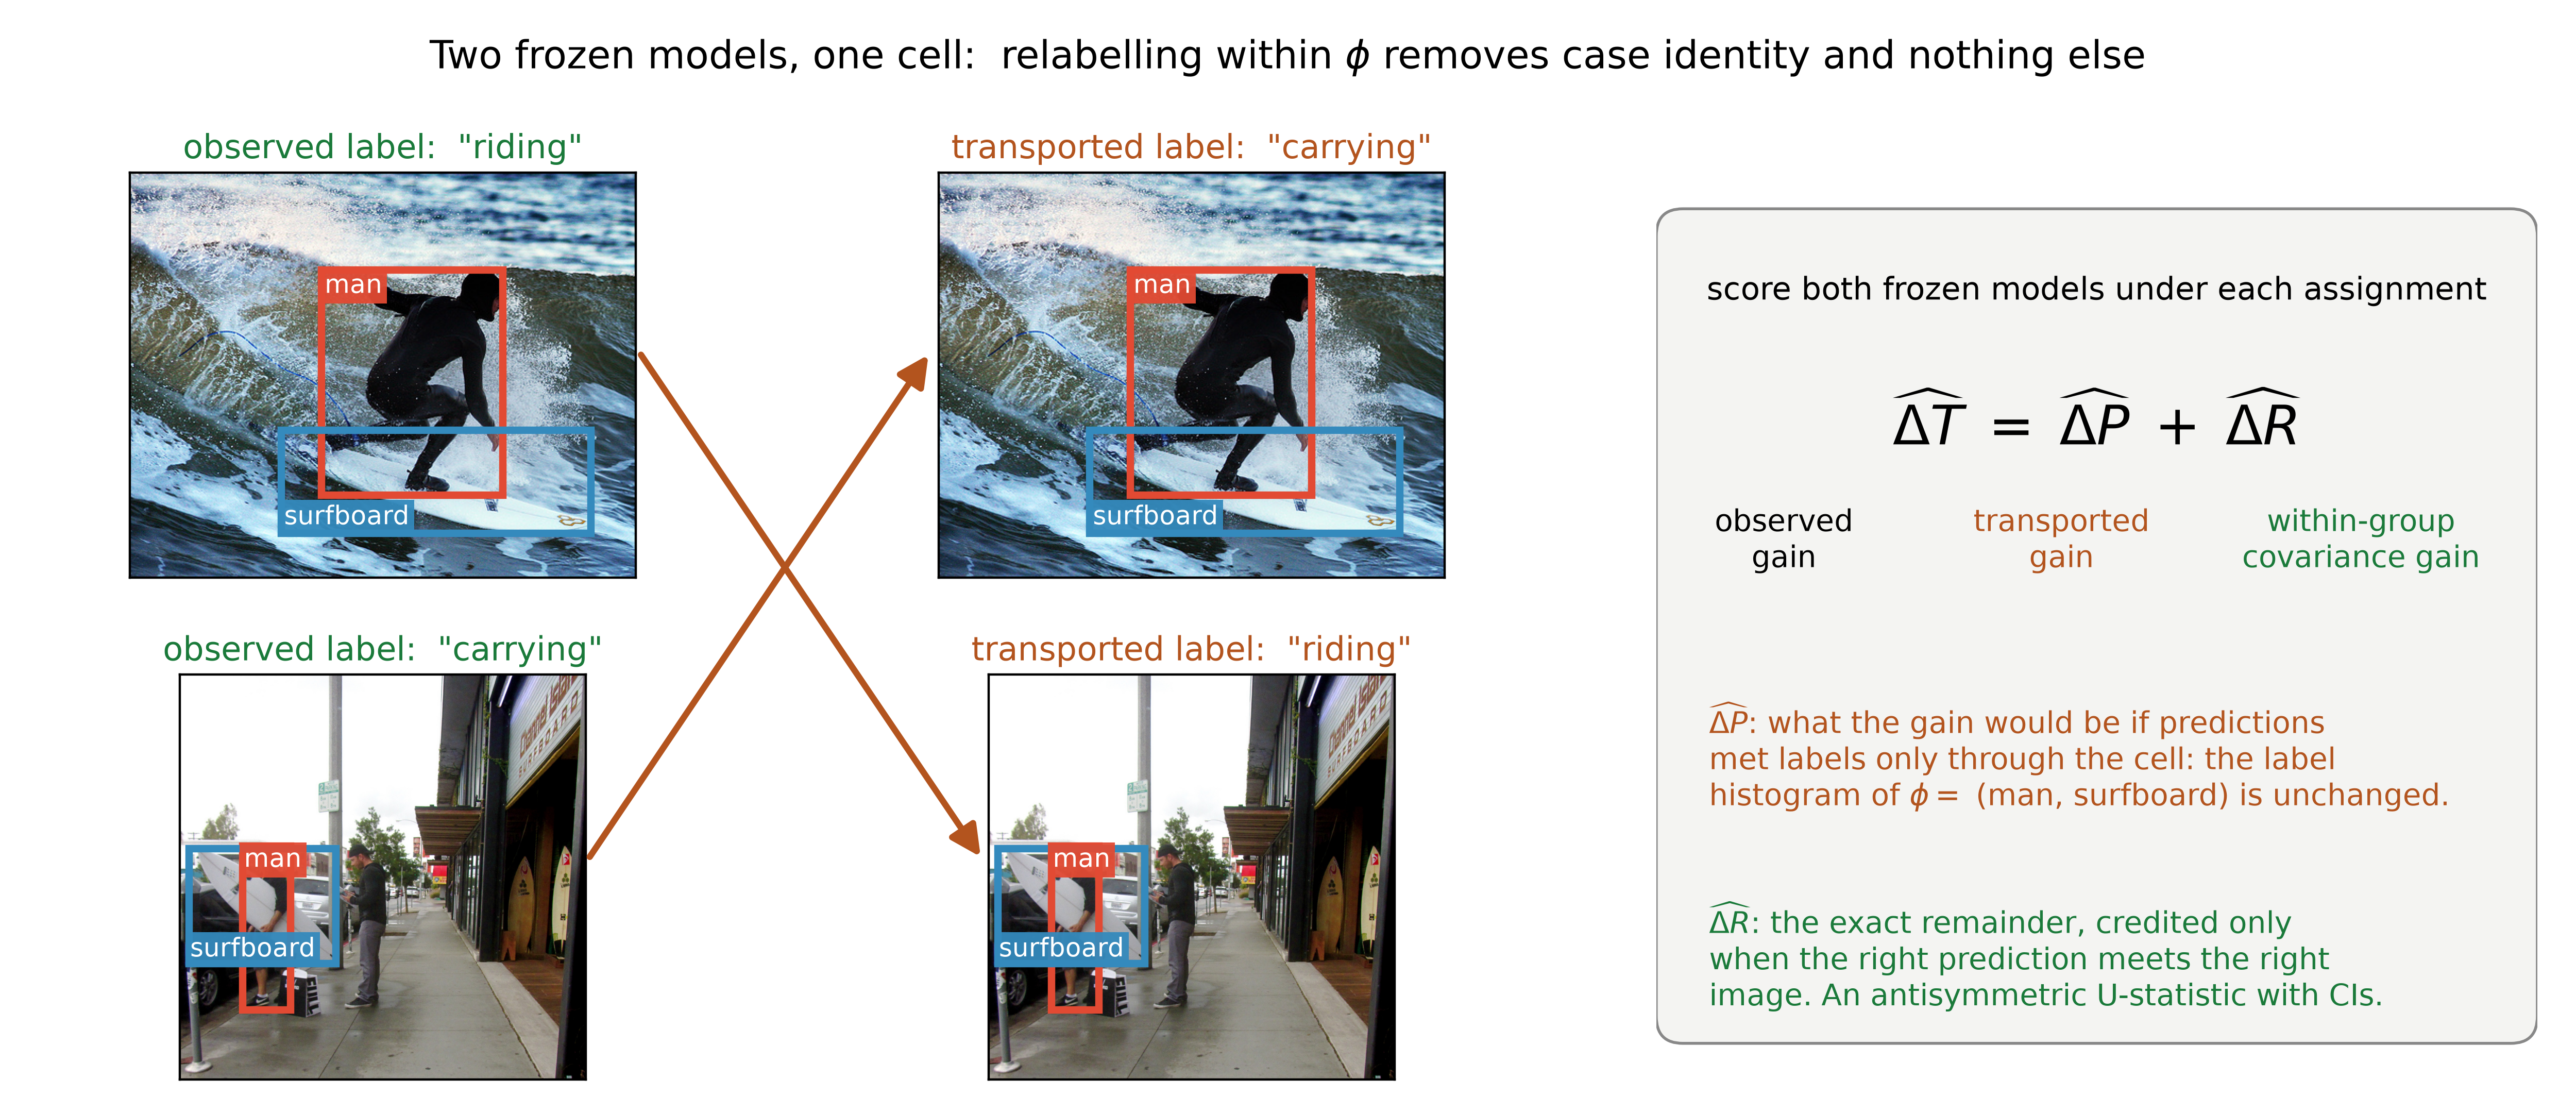
\includegraphics[width=\textwidth]{figures/fig1_new_concept.png}
\caption{\textbf{The construction, on two real test cases.} Two VG150 test relations
share the group $\phi=(\textsf{man},\textsf{surfboard})$ but carry different labels.
Exchanging their labels (arrows) leaves the group and its label frequencies intact while
breaking the link between each prediction and the case it was made for. Scoring two
frozen models before and after the exchange splits their score difference exactly into a
prior-fit gain and a within-group resolution gain.}
\label{fig:concept}
\end{figure*}

\paragraph{What the second component is, in standard terms.}
The surviving component is not a new invention. Written out, the within-group remainder
equals the covariance, inside each group, between how much the new model moved its
predicted probability for a label and whether that label actually occurred
(Theorem~\ref{thm:population}). That covariance is the \emph{resolution} term of the
classical reliability--resolution decomposition of a proper score
\citep{murphy1973vector,degroot1983comparison,brocker2009reliability}, which splits a
single forecaster's score, conditional on a chosen grouping, into how well calibrated it
is and how much its forecasts vary with the outcome. Our contribution is to obtain that
term for a \emph{pair} of forecasters directly, as an exact finite-sample identity with
inference attached, rather than by decomposing each forecaster separately and
subtracting. We call the resulting estimator WAGER (within-group antisymmetric gain
evaluation of resolution) for reference, and name its two components the
\emph{prior-fit gain} and the \emph{within-group resolution gain} throughout.

\subsection{Contributions}\label{sec:contributions}

\begin{enumerate}
\item \textbf{An exact decomposition, and what its remainder is.} For any score, the
observed gain between two frozen models splits exactly --- in the population
(Theorem~\ref{thm:population}) and in the finite sample (Theorem~\ref{thm:sample}) ---
into a prior-fit gain and a remainder that is a U-statistic of order two. For every
Bregman score, and hence for the quadratic and logarithmic scores as named cases, that
remainder equals a within-group covariance between the models' predicted-probability
difference and the label indicator (Theorem~\ref{thm:bregman}). A change that is
constant within groups contributes exactly zero to it.

\item \textbf{Inference for the difference, and its large-sample justification.} We
derive the estimator's influence function, which gives cluster-robust confidence
intervals in one pass over the data, together with a randomization test stratified by
group. The dataset-level estimator is asymptotically normal with a consistent sandwich
variance (Theorem~\ref{thm:clt}); at a trivial grouping variable it reduces exactly to a
clustered Diebold--Mariano test of the paired score differential
(Corollary~\ref{cor:dm}), so the decomposition delivers what that classical test does
plus the split it does not.

\item \textbf{Two exact statements about design choices that would otherwise be
guesswork.} Using a group's own observed label frequency as the counterfactual, rather
than leaving each case out, attenuates the estimate by exactly $(n_c-1)/n_c$ in a group
of size $n_c$ (Proposition~\ref{prop:attenuate}) --- which is why no held-out fold is
needed. Merging groups shifts the estimand by an explicit between-group covariance of
either sign (Proposition~\ref{prop:coarsen}), so a coarser grouping variable cannot be
assumed harmless. A Cauchy--Schwarz bound
(Proposition~\ref{prop:sensitivity}) limits how far an unrecorded grouping variable could
move the reported remainder, from a single elicited correlation.

\item \textbf{Validation, and an audit of a published method.} Simulations establish
interval coverage under clustering and delimit what the two components separate:
prior-only improvements stay out of the resolution component, unrecorded within-group
signal enters it, and monotone recalibration moves score between the components, which is
why we audit calibration-matched pairs. Applied to two publicly released scene-graph
checkpoints --- not to models of our own --- the decomposition shows that a ten-point
improvement in mean recall is overwhelmingly prior-fit under either of two proper scores
(Section~\ref{sec:sggaudit}). Three further studies, in relation prediction and in
long-tailed image and text classification, apply the identical estimator and are reported
in Appendix~\ref{app:studies}.
\end{enumerate}

\subsection{Terminology}\label{sec:terminology}

The construction needs few new words, and Table~\ref{tab:terms} fixes them against their
standard statistical counterparts. Readers who prefer the standard vocabulary can read
``group'' for cell, ``resolution'' for the second component, and ``relabelling within
groups'' for transport, and lose nothing.

\begin{table}[t]
\centering
\small
\caption{The paper's vocabulary, and what it corresponds to in standard terms.}
\label{tab:terms}
\begin{tabular}{@{}p{0.24\textwidth}p{0.30\textwidth}p{0.38\textwidth}@{}}
\toprule
Term used here & Standard counterpart & Meaning \\
\midrule
grouping variable $\phi$ &
stratifying / conditioning variable &
a discrete function of the input, declared before the audit, whose levels the labels
depend on \\
cell $c$ &
level of $\phi$; stratum &
the set of test cases sharing one value of $\phi$ \\
label transport &
within-stratum relabelling; permutation within blocks &
replacing a case's label with another case's label from the same cell \\
total gain $\Delta T$ &
paired score differential &
the observed mean score of the new model minus that of the old \\
prior-fit gain $\Delta P$ &
--- &
the part of $\Delta T$ that survives label transport \\
within-group resolution gain $\Delta R$ &
resolution difference \citep{murphy1973vector,brocker2009reliability} &
the part destroyed by transport; a within-cell prediction--label covariance \\
coverage &
identified fraction &
share of test cases in cells of size $\ge2$, the only cells in which $\Delta R$ is
identified \\
calibration-matched &
temperature-scaled on held-out data &
both models rescaled to comparable confidence before the audit \\
\bottomrule
\end{tabular}
\end{table}

\subsection{Scope, and what is not claimed}\label{sec:scope}

The estimator needs exactly four aligned arrays: two $N\times K$ matrices of predicted
probabilities, the $N$ observed labels, and the $N$ cell identifiers. Any closed-set
probabilistic prediction task supplies them. Free-form or generative evaluation, where no
$K$-way probability vector exists, does not, and we make no claim there.

Three limits on interpretation are worth stating before any result. First, everything is
conditional on the declared $\phi$: a positive $\Delta R$ says the new model predicts
individual cases better \emph{among cases sharing that feature}, and nothing about
causality, reasoning, or robustness. Second, $\Delta R$ credits any signal that varies
within a cell, including a shortcut the analyst did not record;
Proposition~\ref{prop:sensitivity} bounds that exposure rather than removing it. Third, a
prior-fit gain is not illegitimate --- fitting the deployment label distribution better
is real skill whenever that distribution is the one that matters. The decomposition says
where a gain lives, not whether it is worth having.

\paragraph{Organization.}
Section~\ref{sec:worked} works a four-point example. Section~\ref{sec:related} places the
construction in the literature on proper-score decomposition and forecast comparison.
Section~\ref{sec:method} develops the estimator and its theory.
Section~\ref{sec:exp} validates it and audits two released checkpoints.
Sections~\ref{sec:discussion} and~\ref{sec:conclusion} discuss limits and conclude.
Proofs are in Appendix~\ref{app:proofs}; three further empirical studies are in
Appendix~\ref{app:studies}.
